\documentclass[11pt]{article}
\usepackage[layoutsize={8.5in,11in},margin=1in]{geometry}\usepackage{soul}\usepackage{graphicx}\usepackage{amsmath}\usepackage{amssymb}\usepackage{amsthm}\usepackage{mathrsfs}\usepackage{bm}\usepackage{pifont}\usepackage[dvipsnames,svgnames,x11names]{xcolor}\usepackage{setspace}\usepackage{pdfcomment}\usepackage{indentfirst}\usepackage{float}\usepackage{braket}\usepackage{enumerate}\usepackage{tikz}\usetikzlibrary{decorations.pathmorphing,decorations.text,shapes.geometric,3d,positioning,arrows.meta}\usepackage{fontawesome}\usepackage{alltt}\usepackage{pmboxdraw}\usepackage{listings}\usepackage{cleveref}
\def\d{\displaystyle}\def\({\left(}\def\){\right)}\def\[{\left[}\def\]{\right]}\def\L{\left\{}\def\R{\right\}}\def\|{\middle\vert}\def\c{\cdot}\def\cs{\cdots}\def\<={\leq}\def\>={\geq}\def\f{\frac}\def\mrm{\mathrm}\def\bM{\begin{pmatrix}}\def\eM{\end{pmatrix}}\def\lp{\left<}\def\rp{\right>}\def\la{\left|}\def\ra{\right|}\def\lv{\left\Vert}\def\rv{\right\Vert}\def\o{\overline}\def\eps{\varepsilon}\def\E{\mathop{\mathbb{E}}}\def\Pr{\mathop{\mathrm{Pr}}}\def\Var{\mathop{\mathrm{Var}}}\def\|{\middle\vert}\def\b{\mathbf}\def\Re{\mathop{\mrm{Re}}}\def\Im{\mathop{\mrm{Im}}}\def\msf{\mathsf}\def\tsf{\textsf}\def\poly{\mathop{\text{\rm poly}}}\def\wtilde{\widetilde}\def\lf{\left\lfloor}\def\rf{\right\rfloor}\def\lF{\left\lceil}\def\rF{\right\rceil}\def\|{\middle\vert}
\newcommand{\rmnum}[1]{\romannumeral#1}\newcommand{\Rmnum}[1]{\uppercase\expandafter{\romannumeral#1}}\newcommand{\tops}[2]{\texorpdfstring{#1}{#2}}
\newtheorem{theorem}{Theorem}[section]\newtheorem{lemma}[theorem]{Lemma}\newtheorem{definition}[theorem]{Definition}\newtheorem{proposition}[theorem]{Proposition}\newtheorem{corollary}[theorem]{Corollary}\newtheorem{openproblem}[theorem]{Open Problem}\newenvironment{Proof}{\begin{proof}~\par}{\end{proof}}\newenvironment{Solution}{\begin{proof}[Solution]~\par}{\end{proof}}
\mathchardef\standardl=\mathcode`l \mathcode`l=\ell \newcommand{\deactivatel}{\mathcode`l=\standardl} \makeatletter \edef\operator@font{\operator@font\noexpand\deactivatel} \makeatother
\ExplSyntaxOn\NewDocumentCommand{\spreadwords}{m}{\tl_set:Nn\l_tmpa_tl{#1}\tl_replace_all:Nnn\l_tmpa_tl{~}{\hspace{\stretch{1}}}\tl_use:N\l_tmpa_tl}\ExplSyntaxOff

% Set monospace font with Unicode support
\setmonofont{DejaVu Sans Mono}%[Scale=0.85]

%%%%%%%%%%%%%%%%%%%%%%%%%%%%%%%%%%%%%%%%%%%%%%%%%%%%%%%%%%%%%%%%%%%%%

\title{Datapack: Bundle-Based RuneForge System}
\author{\tt Lj\_1}
\date{\today}

\begin{document}

\maketitle
\tableofcontents

\section{Player Guide}

When placing tools or armor (referred to as \textit{items}) in the $2 \times 2$ crafting grid, you can modify their \textit{runes} as if they were a bundle. Each \textit{rune} enhances the \textit{item} by adding enchantments, modifying attributes, or granting custom abilities.

% CHANGED: Reworded for conciseness and clarity.
This datapack is designed to be \textbf{collaboration-friendly}: in a collaborative map, each creator can design custom runes without altering the RuneForge system's core code.

\begin{figure}[htbp]
  \centering
  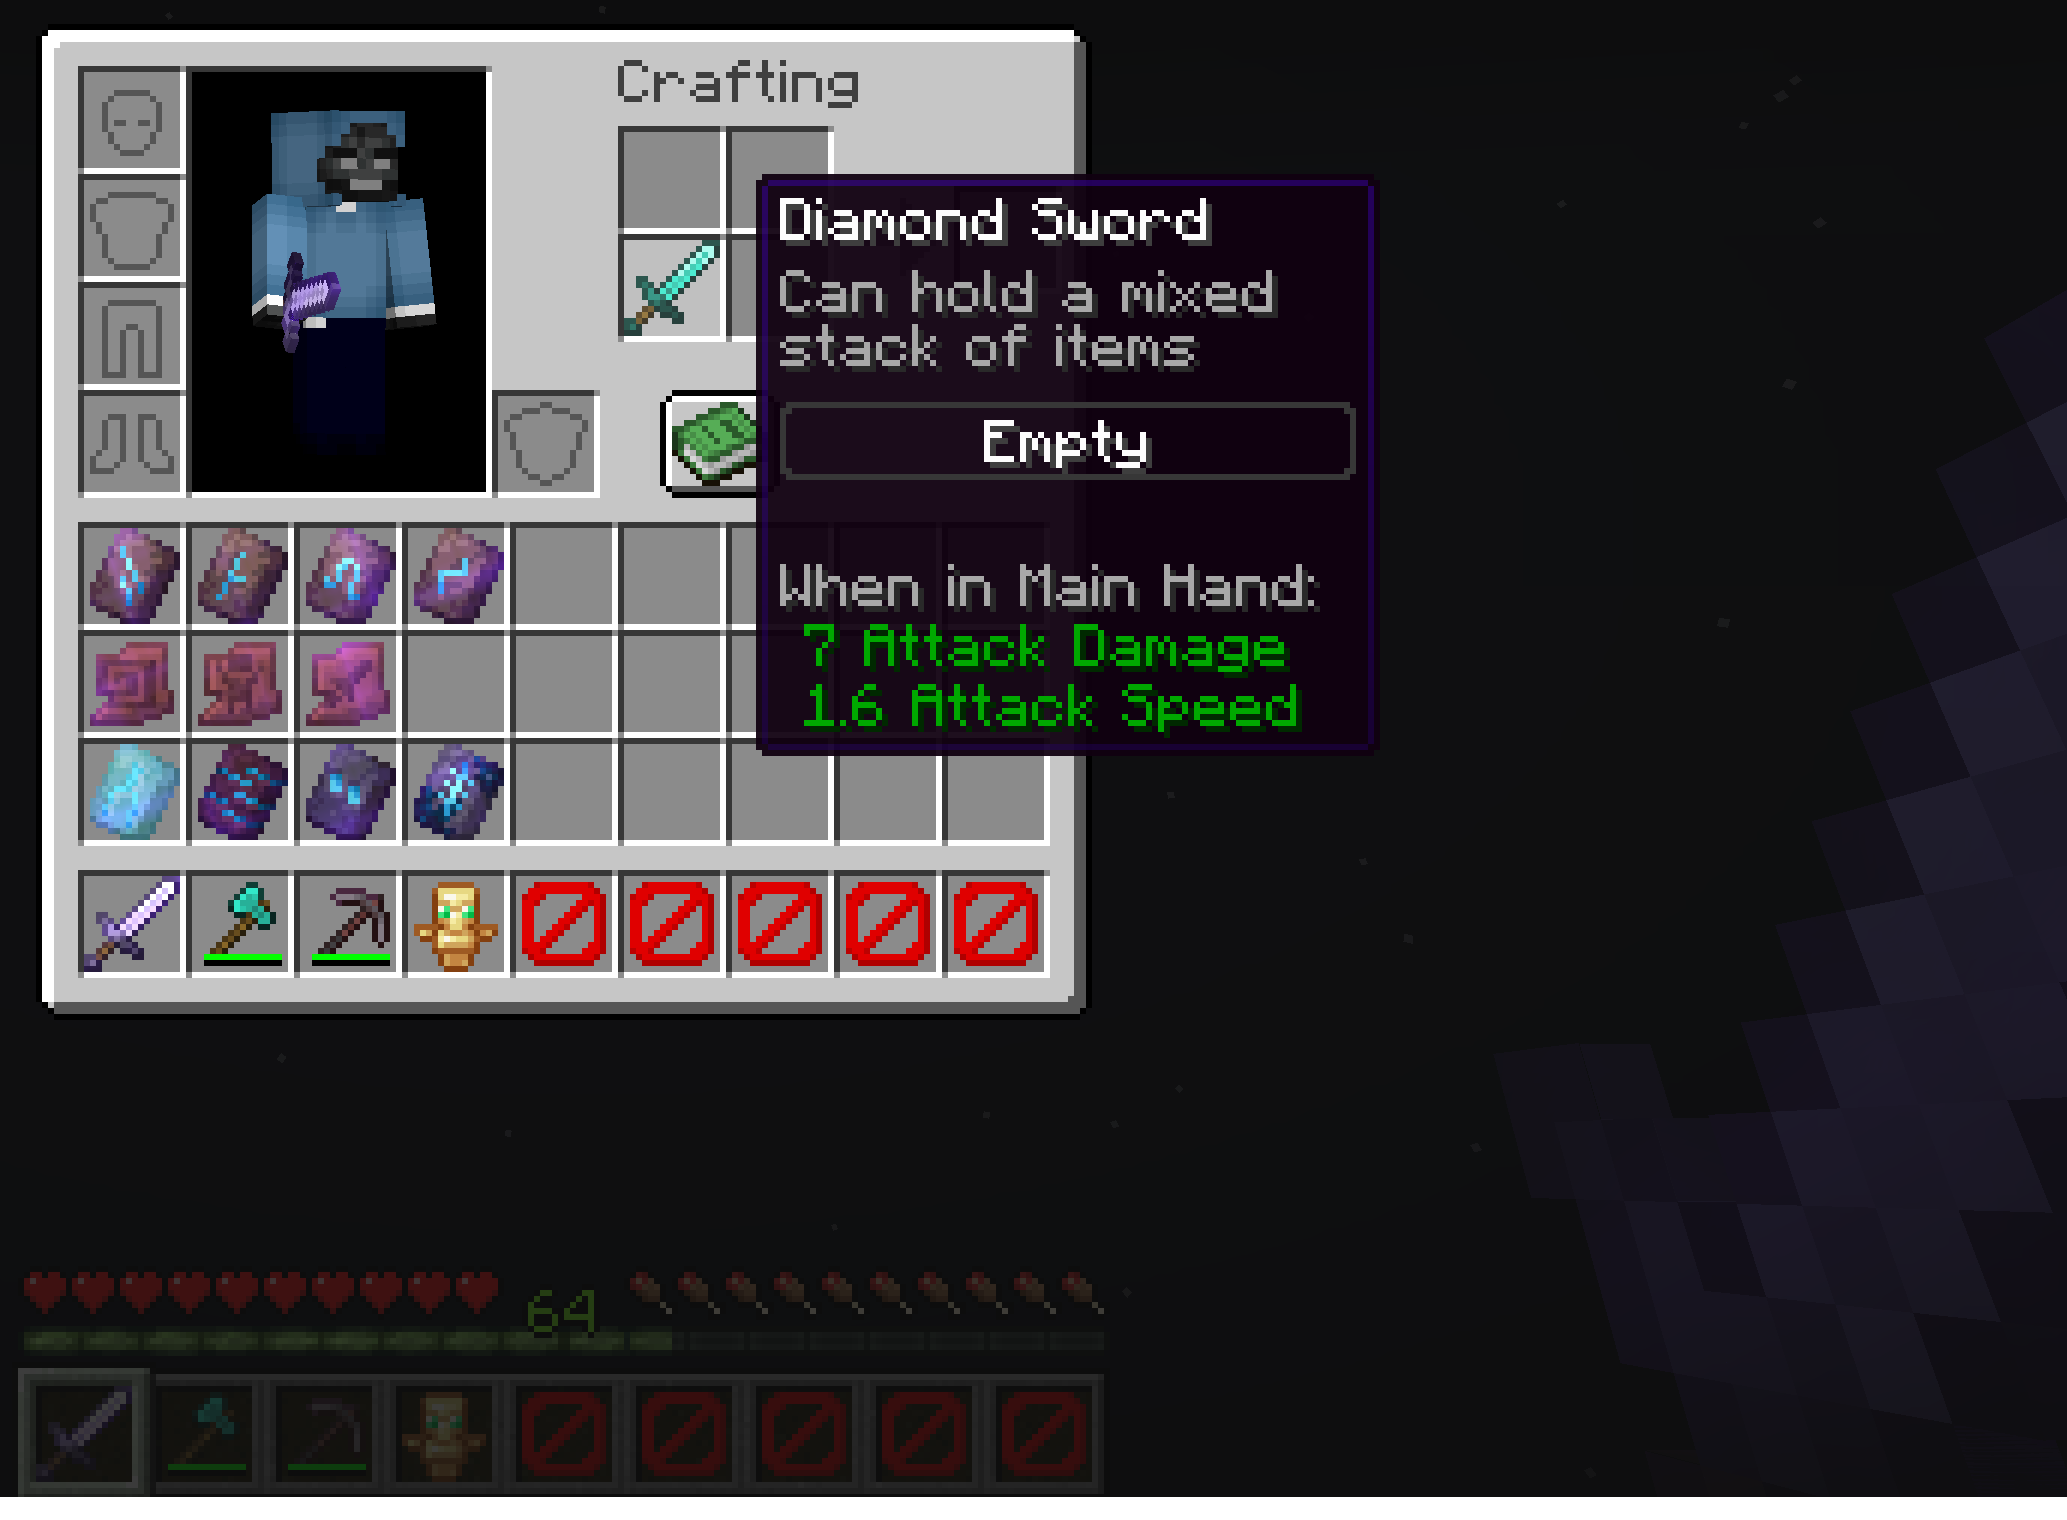
\includegraphics[width=3in]{Screenshot from 2025-04-04 21-44-19.png}
  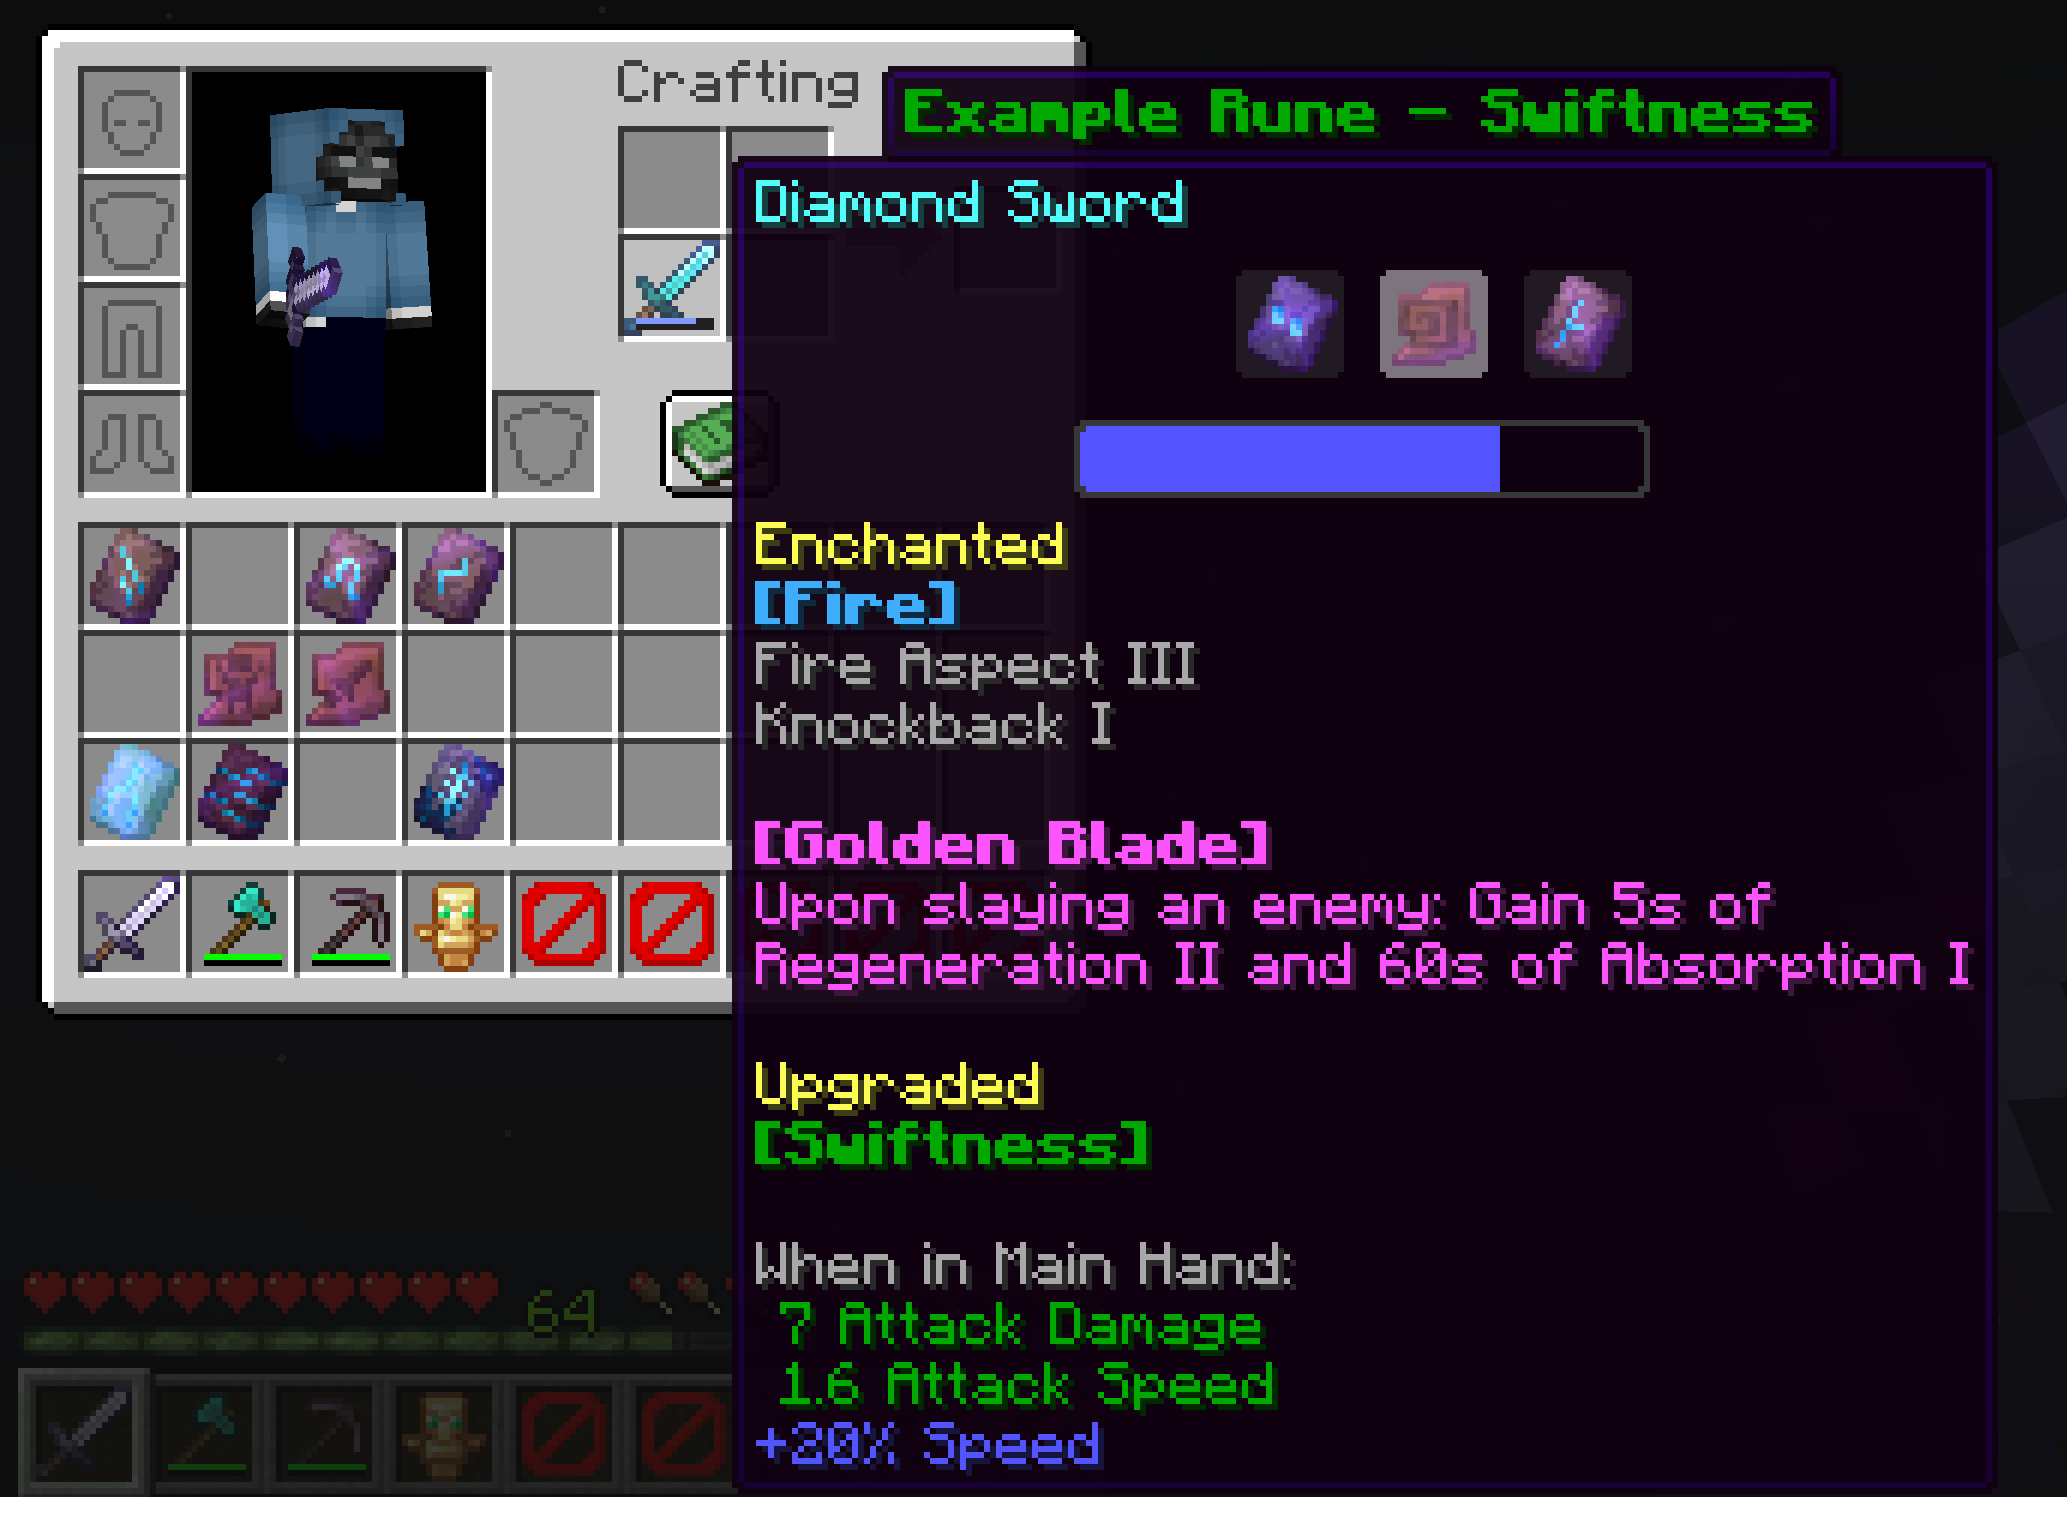
\includegraphics[width=3in]{Screenshot from 2025-04-04 21-48-46.png}
  \caption{Modifying runes on an item (bundle-like interface).} % CHANGED: Simplified caption.
\end{figure}

\begin{figure}[htbp]
  \centering
  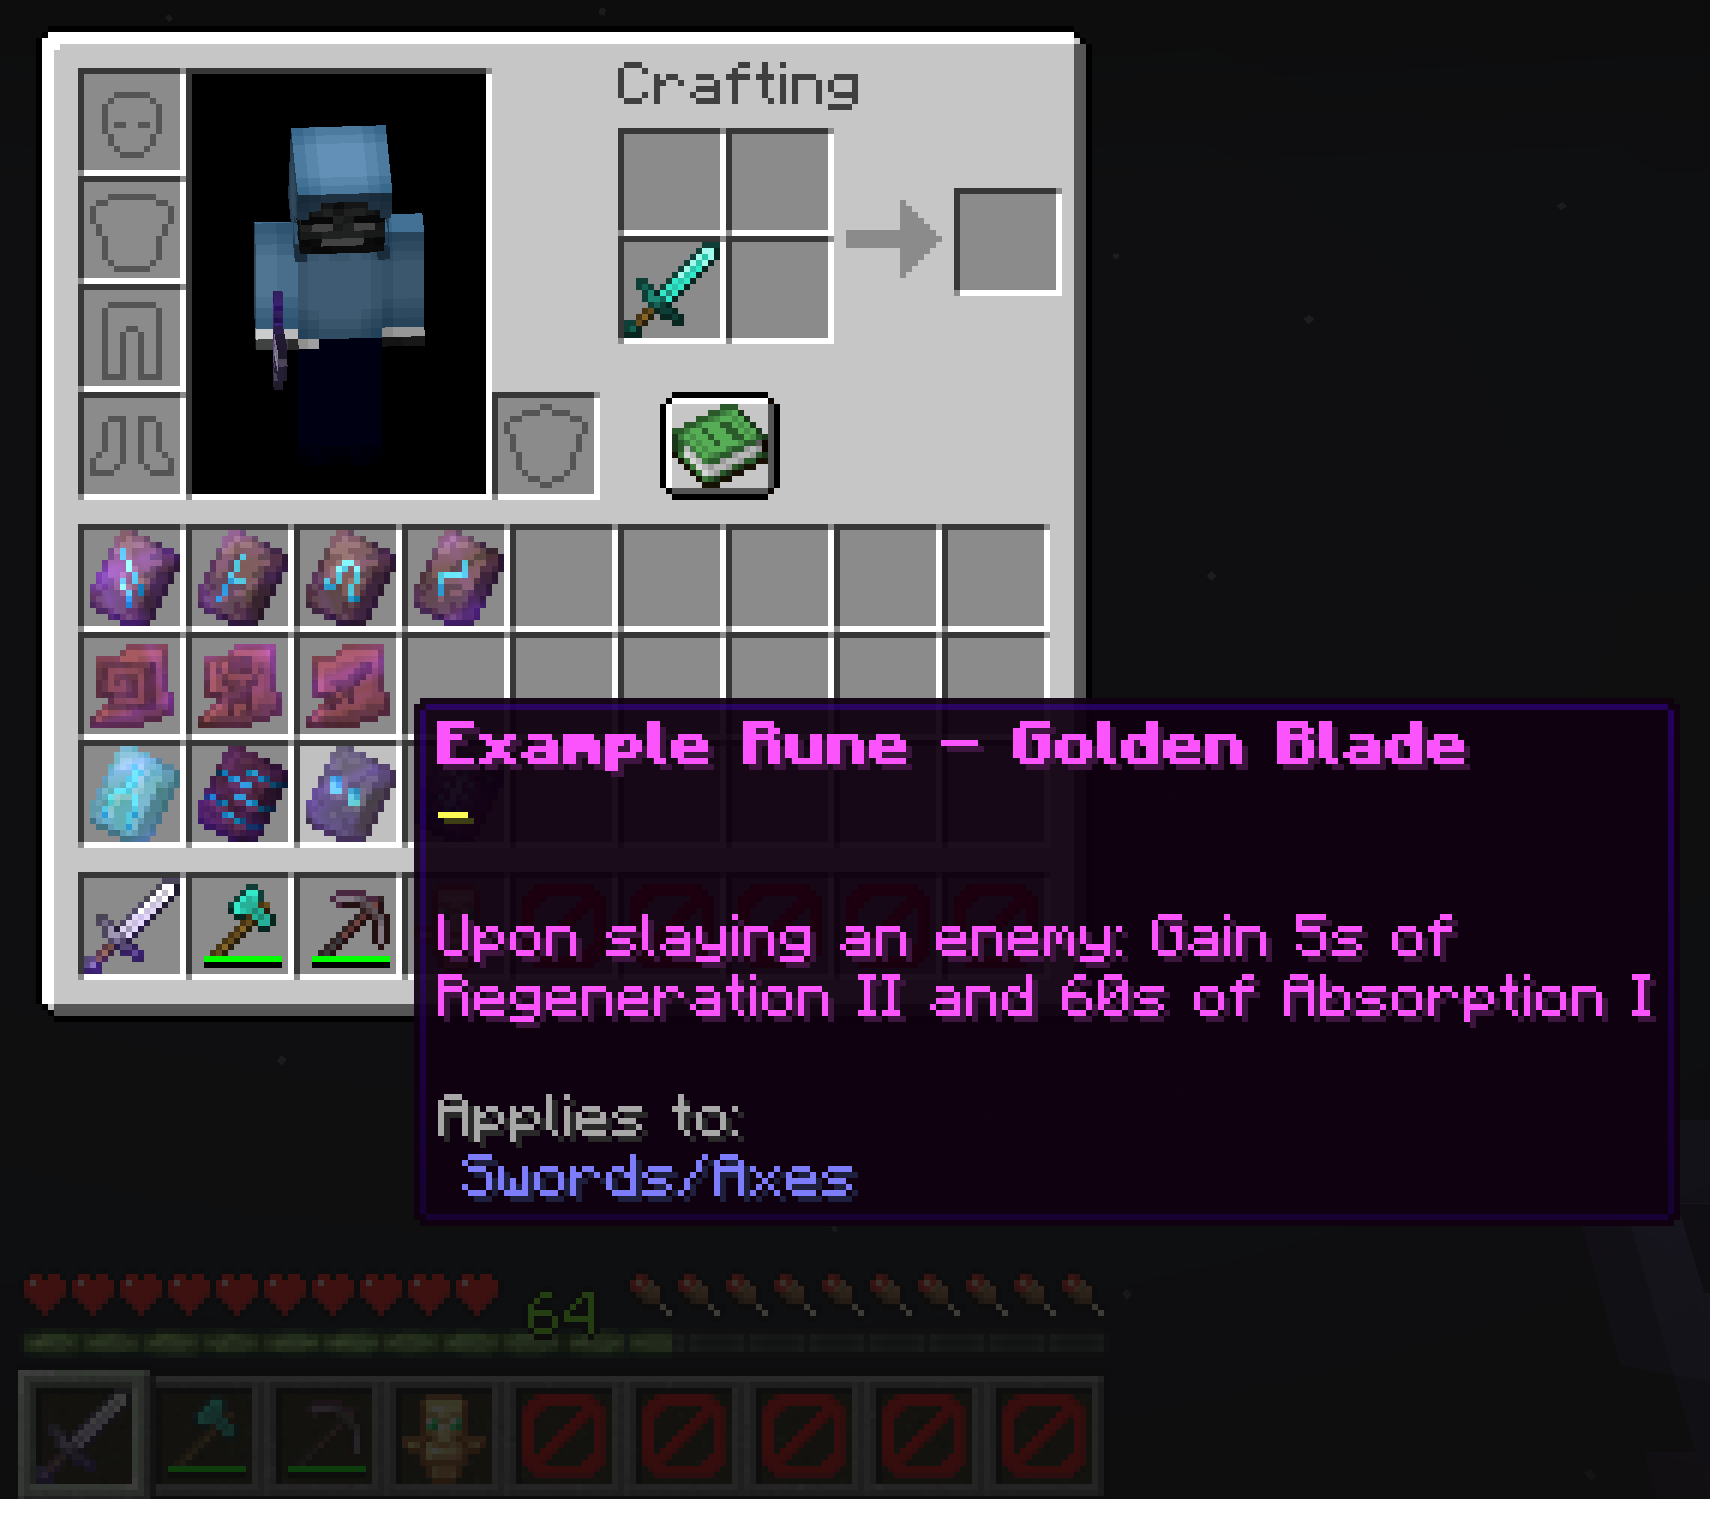
\includegraphics[width=2in]{Screenshot from 2025-04-04 21-55-31.png}
  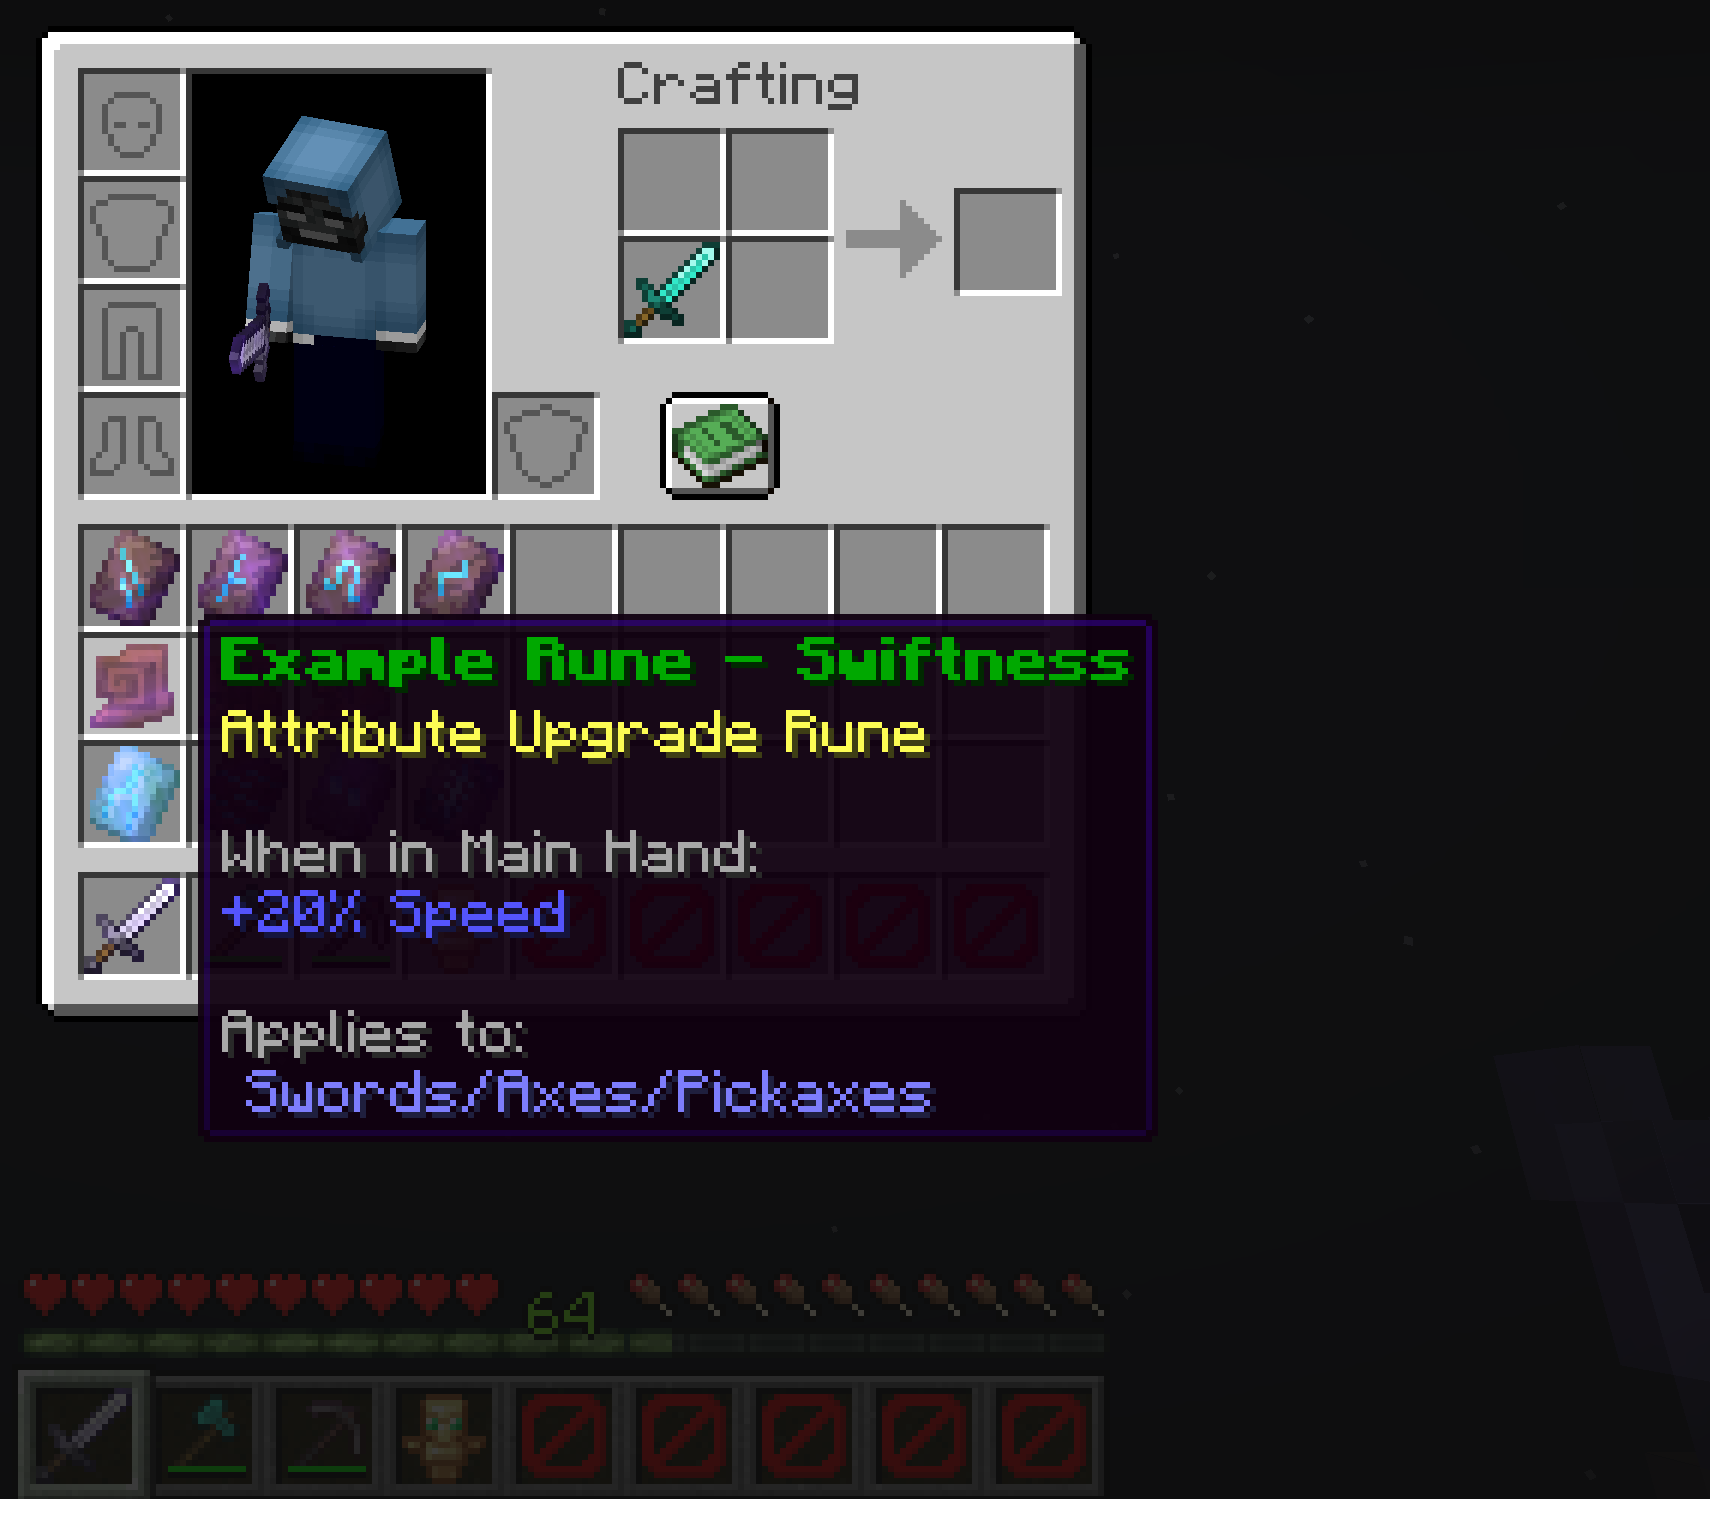
\includegraphics[width=2in]{Screenshot from 2025-04-04 21-55-36.png}
  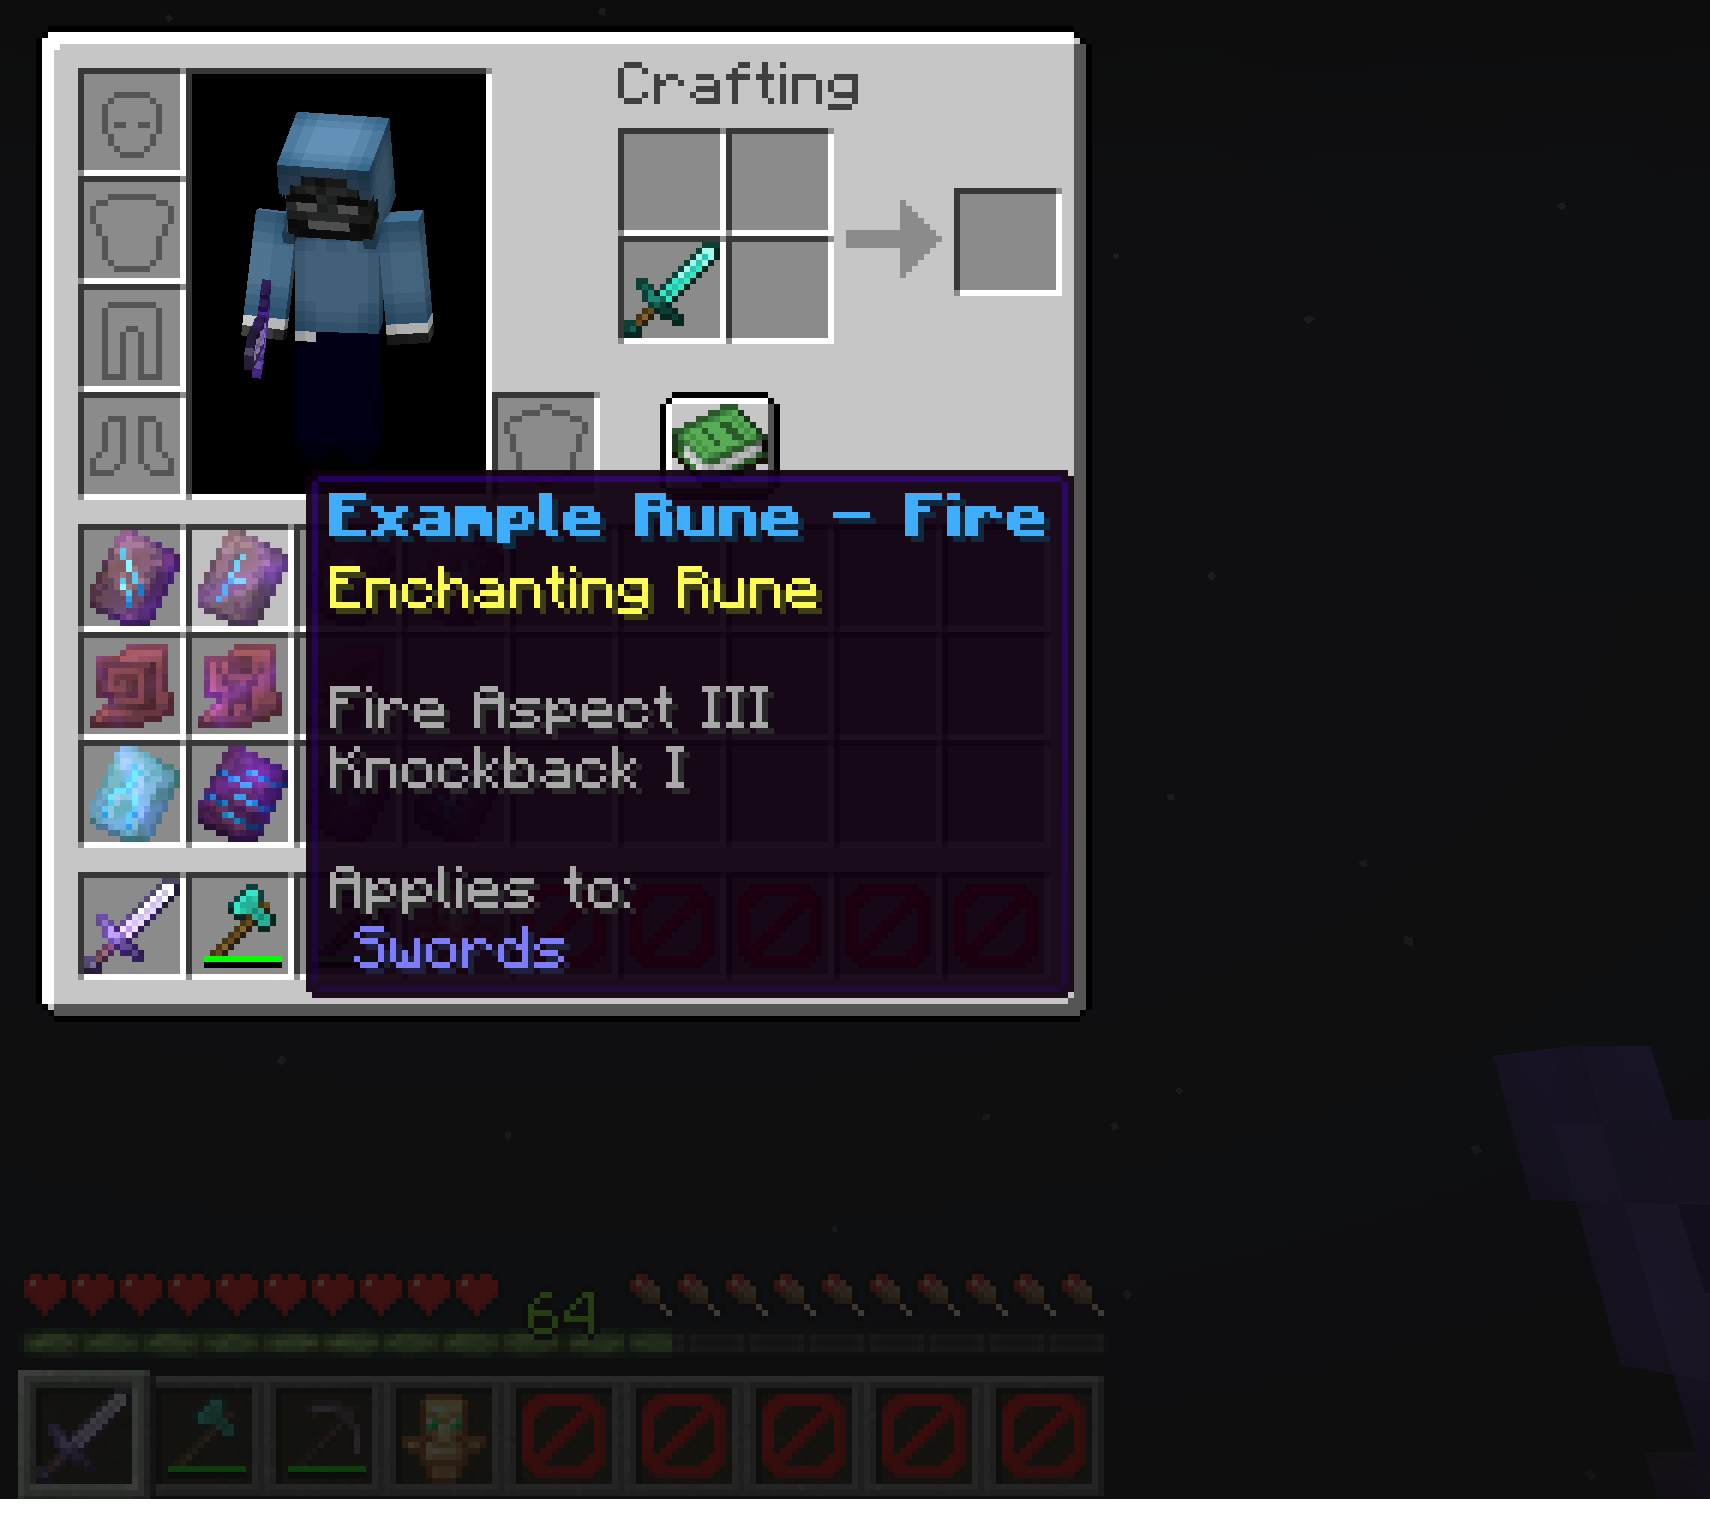
\includegraphics[width=2in]{Screenshot from 2025-04-04 21-55-42.png}
  \caption{Example runes.} % CHANGED: More concise.
\end{figure}

\begin{itemize}
  \item \colorbox{black!20}{\small\tt Lj\_1 - [1.21.5] Bundle-Based RuneForge System} is the core datapack;
  \item \colorbox{black!20}{\small\tt Lj\_1 - [1.21.5] Bundle-Based RuneForge System - Examples} provides\\example runes. Execute \colorbox{black!20}{\small\tt/function lj.bundle\_forge.examples:get\_runes} to obtain them. Also execute \colorbox{black!20}{\small\tt/function lj.core:\_\_install\_\_} to initialize scoreboard objectives.
\end{itemize}

\subsection{More Features}

Each rune occupies $1/k$ (for some integer $k \geq 1$) of the bundle's capacity, limiting the number of runes per item. In the examples, rune weights are color-coded:

\begin{figure}[htbp]
  \centering
  \begin{tabular}{|c|c|}
    \hline
    \textbf{Color} & \textbf{Weight} \\ % CHANGED: Capitalized header.
    \hline
    \colorbox[HTML]{00AA00}{Green} & 1/6 \\ % CHANGED: Capitalized color names.
    \hline
    \colorbox[HTML]{3FAFFF}{Blue} & 1/4 \\
    \hline
    \colorbox[HTML]{FF55FF}{Purple} & 1/3 \\
    \hline
    \colorbox[HTML]{FFAA00}{Gold} & 1/2 \\
    \hline
  \end{tabular}
\end{figure}

\begin{figure}[htbp]
  \centering
  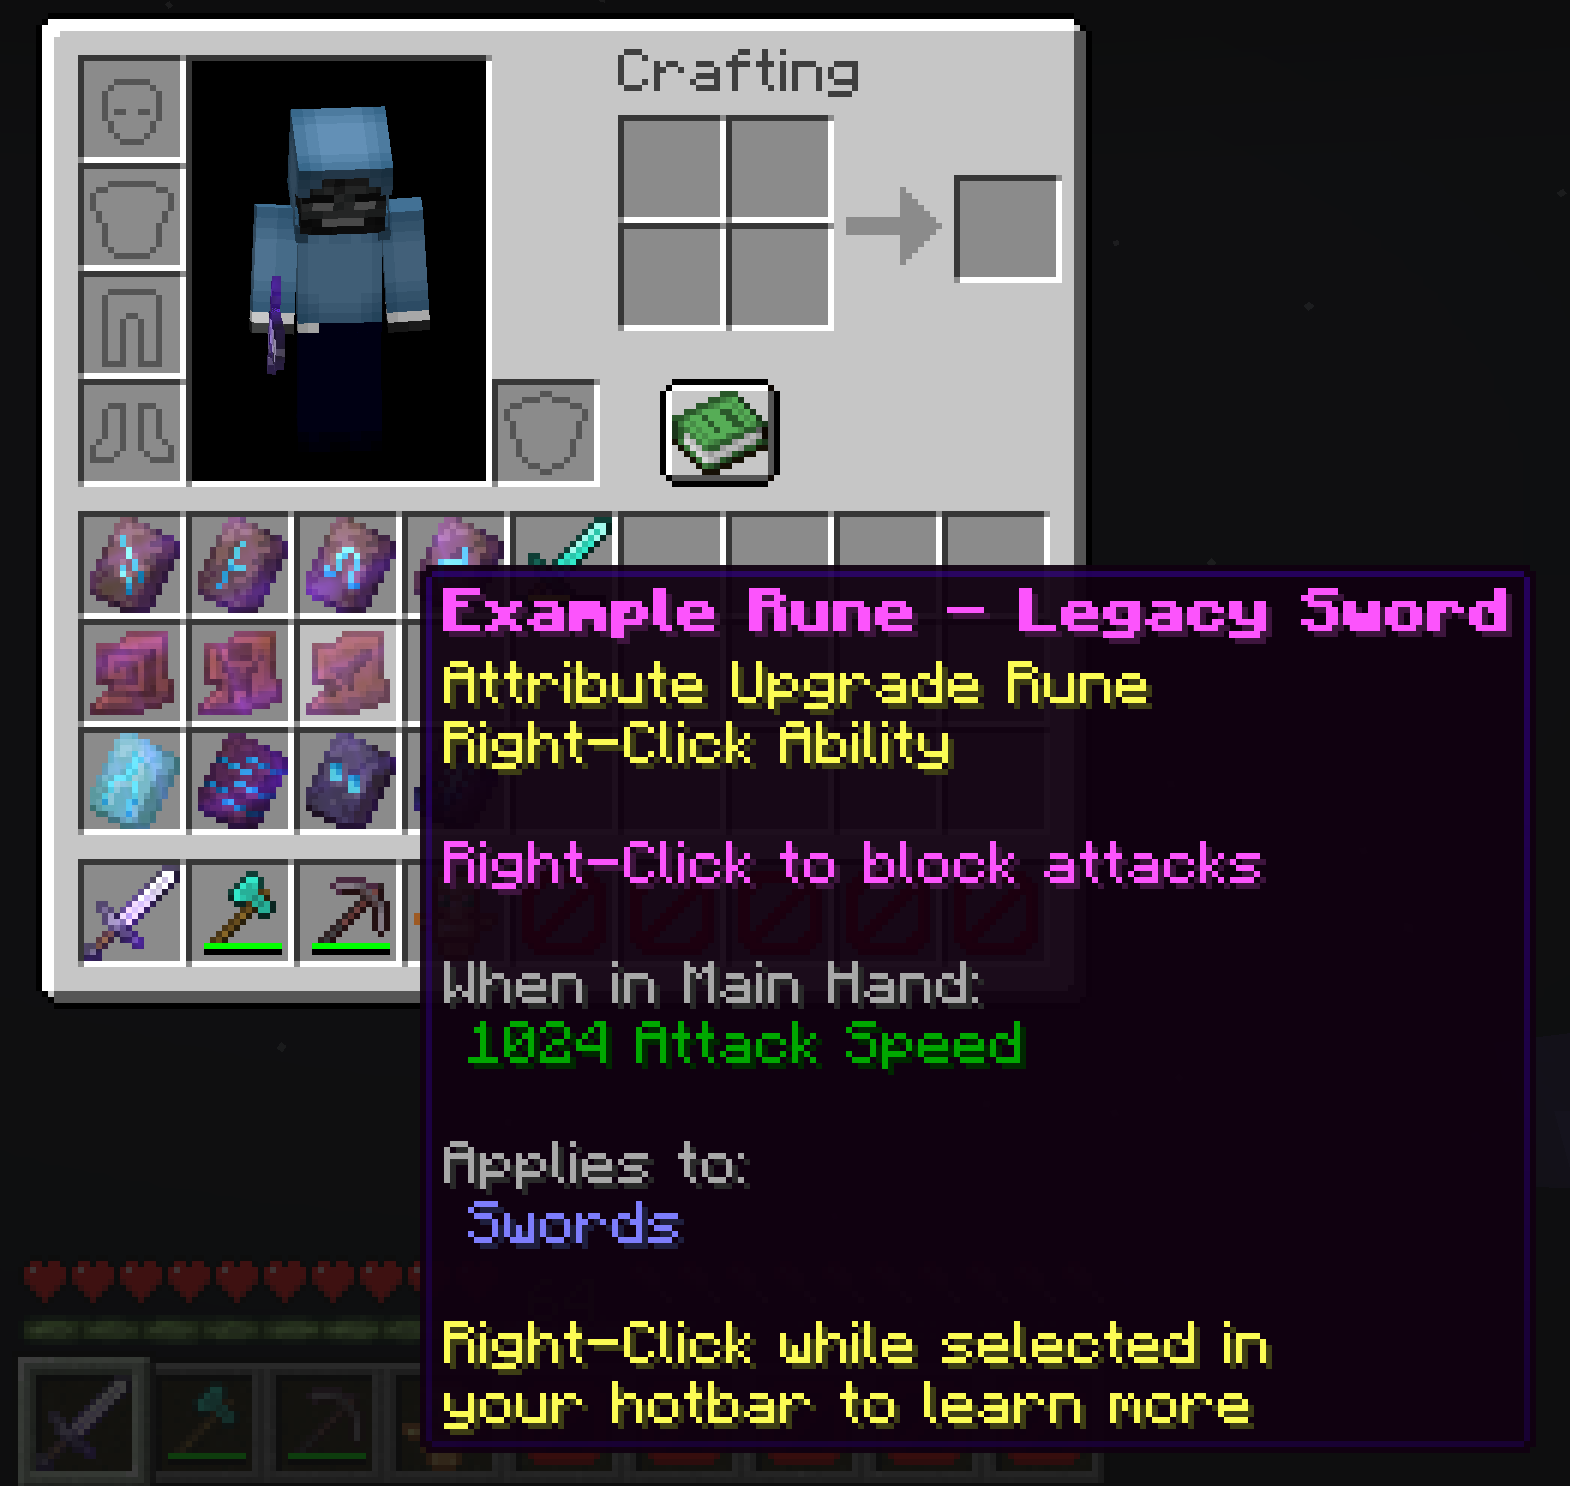
\includegraphics[width=2.5in]{Screenshot from 2025-04-04 23-18-59.png}
  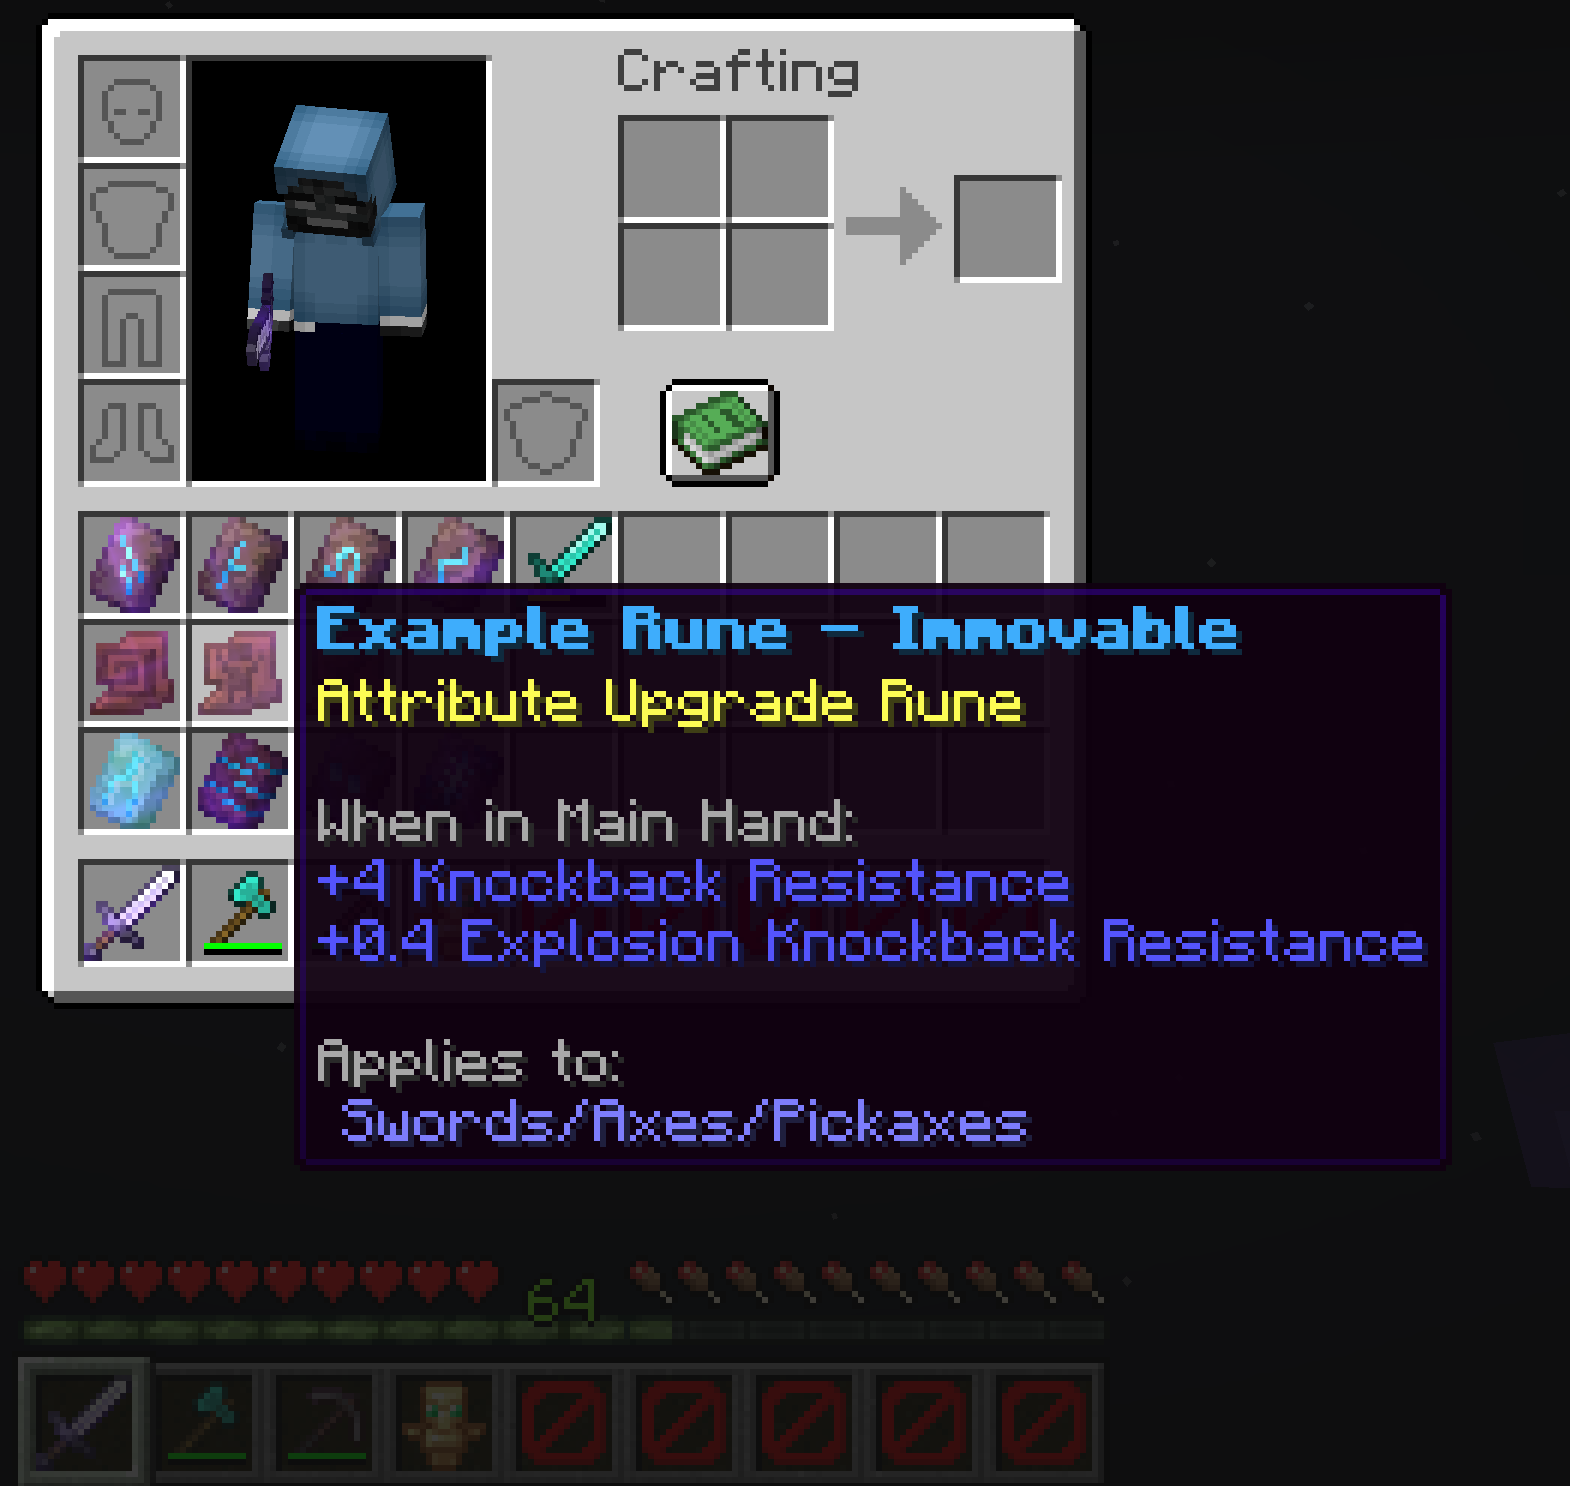
\includegraphics[width=2.5in]{Screenshot from 2025-04-04 23-19-04.png}
  \caption{These runes conflict because both of them are Attribute Upgrade Runes}
\end{figure}

Some runes conflict with each other, which means they cannot be applied to an item simultaneously. In the examples, runes with the same yellow-labeled categories conflict.

When a rune-equipped item breaks, its runes are automatically returned to you.

\subsection{Warnings (IMPORTANT)}

% CHANGED: Reworded for clarity and added durability note.
Other modifications (e.g., from anvils, smithing tables, or enchanting tables) \textbf{may not} persist when using the $2 \times 2$ crafting grid. The RuneForge system calculates results based on the original item, ignoring most external changes. Nevertheless, you can configure which fields persist. See \Cref{sec: cfg} for more details.

\section{Map Maker Guide}

% Symbols and icons
\newcommand{\compound}{\textcolor{blue!70}{\faCube}}
\newcommand{\stringicon}{\textcolor{green!60!black}{\faTag}}
\newcommand{\inticon}{\textcolor{red!70}{\faHashtag}}
\newcommand{\listicon}{\textcolor{purple!70}{\faListOl}}
\newcommand{\byteicon}{\textcolor{orange!70}{\faDotCircleO}}
% Custom box characters for better alignment
\newcommand{\vertline}{\textSFviii\;}
\newcommand{\nodeend}{\textSFx\textSFx\;}
\newcommand{\nodesplit}{\textSFx\textSFii\;}
% text styles
\newfontfamily{\latin}{Latin Modern Math}
\newcommand{\desc}[1]{{\latin #1}}
\newcommand{\key}[1]{{\small\textbf{#1}}}

\subsection{Forgeable Items}

The tag \texttt{\small lj.bundle\_forge:forgeable} determines which items display the bundle interface.

\subsection{Customizing Runes}

\begin{alltt}
  \compound\key{minecraft:custom_data}
  └ \compound\key{lj.bundle_forge:rune}
    ├ \stringicon\listicon\key{supported_items:} \desc{Any number of \href{https://minecraft.wiki/w/Item}{item}(s) (an \href{https://minecraft.wiki/w/Resource_location}{ID}, or a \href{https://minecraft.wiki/w/Enchantment_tag_(Java_Edition)}{tag} with #, or an array}
    │   \desc{containing IDs): Items on which this rune can be applied.}
    ├ \stringicon\compound\listicon\key{modifier:} \desc{(Optional) An \href{https://minecraft.wiki/w/Item_modifier}{item modifier} that is applied to the item.}
    ├ \stringicon\key{function:} \desc{(Optional) Execute a function to perform more complicated item}
    │   \desc{modifications. The target item is accessible at{\small\tt entity @s equipment.mainhand}.}
    └ \listicon\key{exclusive_classes:} \desc{(Optional) A list of strings. Runes or items whose}
        \desc{exclusive classes intersect are incompatible with each other.}
  \compound\key{minecraft:max_stack_size:} \desc{Controlls the weight of this rune.}
\end{alltt}

Also customize \texttt{\small minecraft:item\_name}, \texttt{\small minecraft:lore}, etc., for visual polish.

\subsection{Customizing Items}

\begin{alltt}
  \compound\key{minecraft:custom_data}
  └ \compound\key{lj.bundle_forge:item}
    ├ \compound\key{base:} \desc{(Optional) An item stack: This item's ID, count, components without runes}
    │   \desc{applied. Automatically filled if omitted.}
    └ \listicon\key{exclusive_classes:} \desc{(Optional) A list of strings. Runes or items whose}
        \desc{exclusive classes intersect are incompatible with each other.}
\end{alltt}

\subsection{Configuration}\label{sec: cfg}

\begin{alltt}
  \compound\key{lj.bundle_forge:config}
  ├ \listicon\key{persist_fields:} \desc{A list of NBT paths: external changes to these fields persist in the}
  │   \desc{forging system. E.g., {\small\tt ['id','components."minecraft:damage"','components.}}
  │   \desc{{\small\tt"minecraft:custom_data".skill_cd']}.}
  ├ \stringicon\key{final_function:} \desc{(Optional) Executes a function after all rune modifications are applied.}
  └ \compound\key{error_msg_ir}
    └ \stringicon\compound\listicon\textit{\key{<key>:}} \desc{A \href{https://minecraft.wiki/w/Text_component_format}{text component}: The error message displayed when trying to apply a}
        \desc{rune to an item that both have {\tt\small<key>} in their {\tt\small{exclusive_classes}}.}
\end{alltt}

\begin{center}
  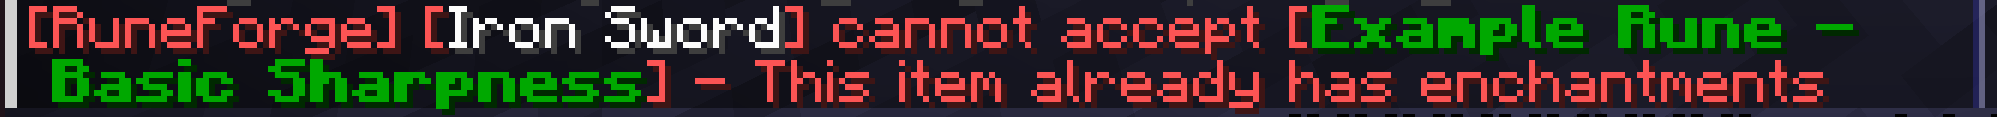
\includegraphics[width=6in]{Screenshot from 2025-04-04 23-39-41.png}
\end{center}

\subsection{Examples}

% CHANGED: Added introductory notes for commands.
The following command grants a rune that applies {\small\tt Sharpness I} to swords:

\lstset{
  breaklines=true,
  basicstyle=\ttfamily\small,
  keepspaces=true,
  showspaces=false
}
\begin{lstlisting}
    /give @s minecraft:written_book[minecraft:custom_data={"lj.bundle_forge:rune":{supported_items:"#minecraft:enchantable/sword",modifier:{function:"minecraft:set_enchantments",enchantments:{"minecraft:sharpness":1}},exclusive_classes:["enchant"]}},minecraft:max_stack_size=6]
\end{lstlisting}

This command creates a rune that sets swords' attack speed to 2.4:

\begin{lstlisting}
    /give @s minecraft:written_book[minecraft:custom_data={"lj.bundle_forge:rune":{supported_items:"#minecraft:enchantable/sword",modifier:{function:"minecraft:set_attributes",modifiers:[{attribute:"minecraft:attack_speed",operation:"add_value",amount:-1.6,id:"minecraft:base_attack_speed",slot:"mainhand"}],replace:false},exclusive_classes:["attribute"]}},minecraft:max_stack_size=6]
\end{lstlisting}

\section*{Acknowledgments} % CHANGED: Corrected spelling.
This datapack is inspired by \href{https://ctmrepository.com/index.php?action=viewMap&id=588}{Ragecraft IV}'s RuneForge system and \href{https://github.com/pearuhdox/Cartographer-2.0}{Cartographer 2.0}'s Encyclopedia.

\appendix

\section{Update Logs}

\begin{itemize}
  \item \textbf{2024-04-28}
    \begin{itemize}
      \item When a rune-equipped item breaks, its runes are automatically returned to you.
    \end{itemize}

  \item \textbf{2024-04-27}
    \begin{itemize}
      \item Fixed some bugs.
    \end{itemize}

  \item \textbf{2024-04-10}
    \begin{itemize}
      \item More complicated item modifications can now be executed through functions.
    \end{itemize}

  \item \textbf{2024-04-08}
    \begin{itemize}
      \item Added persistent fields configuration to support tracking of item durability, netherite upgrade, etc..
    \end{itemize}
  
  \item \textbf{2024-04-05}
    \begin{itemize}
      \item Initial version of Bundle-Based RuneForge System.
    \end{itemize}
\end{itemize}

\end{document}